% Figure 7: ARE vs Known Extractors (grouped bar chart)
\documentclass[tikz,border=5pt]{standalone}
\usepackage{pgfplots}
\pgfplotsset{compat=1.18}

\begin{document}
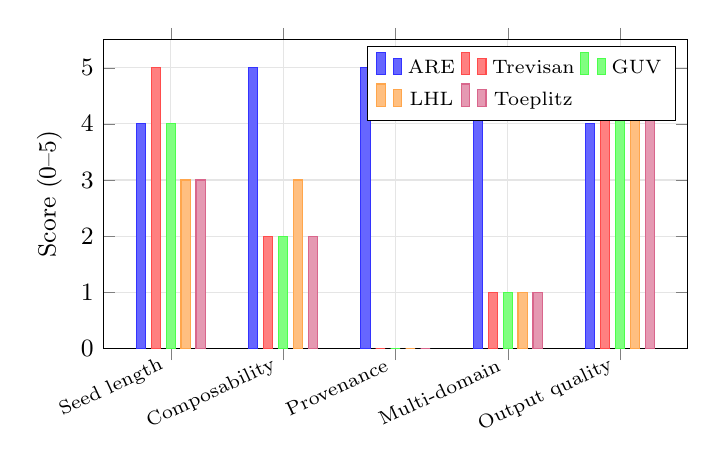
\begin{tikzpicture}
\begin{axis}[
  width=9cm, height=5.5cm,
  ybar,
  bar width=0.12cm,
  enlarge x limits=0.15,
  ylabel={Score (0--5)},
  symbolic x coords={Seed length, Composability, Provenance, Multi-domain, Output quality},
  xtick=data,
  x tick label style={rotate=25, anchor=east, font=\scriptsize},
  ymin=0, ymax=5.5,
  ytick={0,1,2,3,4,5},
  legend style={at={(0.98,0.98)}, anchor=north east, font=\scriptsize, legend columns=3},
  grid=major,
  grid style={gray!20},
  font=\small,
]

% ARE
\addplot[fill=blue!60, draw=blue!80] coordinates {
  (Seed length, 4)
  (Composability, 5)
  (Provenance, 5)
  (Multi-domain, 5)
  (Output quality, 4)
};
\addlegendentry{ARE}

% Trevisan
\addplot[fill=red!50, draw=red!70] coordinates {
  (Seed length, 5)
  (Composability, 2)
  (Provenance, 0)
  (Multi-domain, 1)
  (Output quality, 5)
};
\addlegendentry{Trevisan}

% GUV
\addplot[fill=green!50, draw=green!70] coordinates {
  (Seed length, 4)
  (Composability, 2)
  (Provenance, 0)
  (Multi-domain, 1)
  (Output quality, 5)
};
\addlegendentry{GUV}

% LHL/Universal Hash
\addplot[fill=orange!50, draw=orange!70] coordinates {
  (Seed length, 3)
  (Composability, 3)
  (Provenance, 0)
  (Multi-domain, 1)
  (Output quality, 5)
};
\addlegendentry{LHL}

% Toeplitz
\addplot[fill=purple!40, draw=purple!60] coordinates {
  (Seed length, 3)
  (Composability, 2)
  (Provenance, 0)
  (Multi-domain, 1)
  (Output quality, 5)
};
\addlegendentry{Toeplitz}

\end{axis}
\end{tikzpicture}
\end{document}
